% Created by tikzDevice version 0.12.6 on 2024-10-10 10:16:23
% !TEX encoding = UTF-8 Unicode
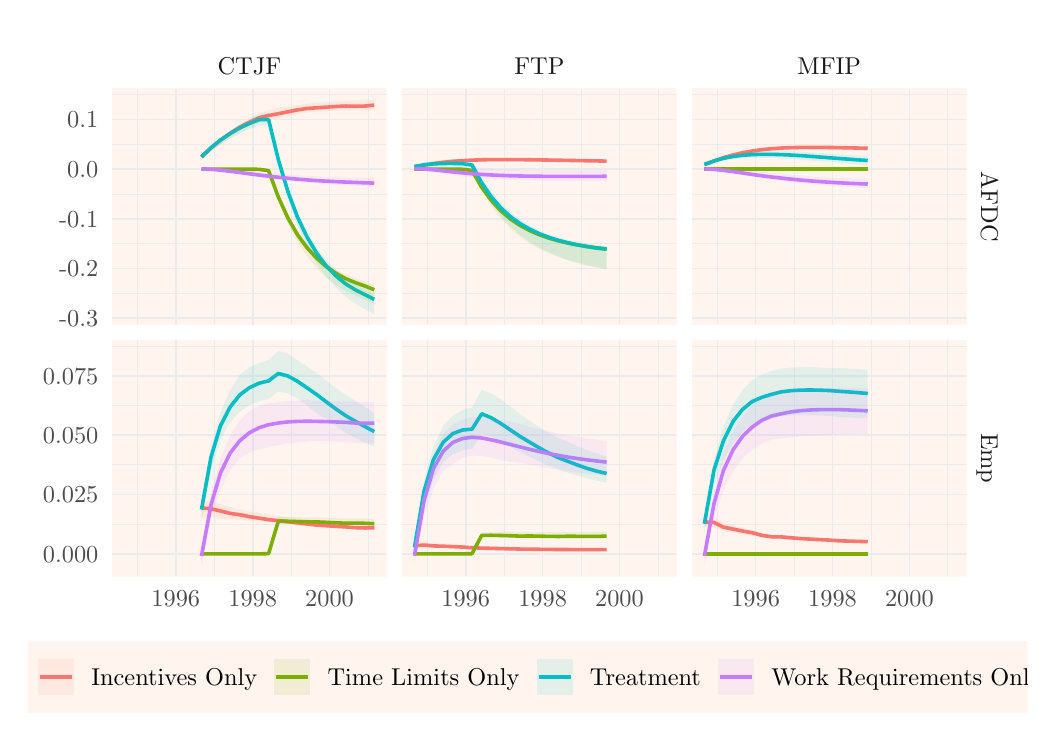
\begin{tikzpicture}[x=1pt,y=1pt]
\definecolor{fillColor}{RGB}{255,255,255}
\path[use as bounding box,fill=fillColor,fill opacity=0.00] (0,0) rectangle (361.35,252.94);
\begin{scope}
\path[clip] ( 30.49,145.52) rectangle (129.75,230.87);
\definecolor{drawColor}{RGB}{255,245,238}
\definecolor{fillColor}{RGB}{255,245,238}

\path[draw=drawColor,line width= 0.6pt,line join=round,line cap=round,fill=fillColor] ( 30.49,145.52) rectangle (129.75,230.87);
\definecolor{drawColor}{gray}{0.92}

\path[draw=drawColor,line width= 0.3pt,line join=round] ( 30.49,156.90) --
	(129.75,156.90);

\path[draw=drawColor,line width= 0.3pt,line join=round] ( 30.49,174.86) --
	(129.75,174.86);

\path[draw=drawColor,line width= 0.3pt,line join=round] ( 30.49,192.82) --
	(129.75,192.82);

\path[draw=drawColor,line width= 0.3pt,line join=round] ( 30.49,210.79) --
	(129.75,210.79);

\path[draw=drawColor,line width= 0.3pt,line join=round] ( 30.49,228.75) --
	(129.75,228.75);

\path[draw=drawColor,line width= 0.3pt,line join=round] ( 39.64,145.52) --
	( 39.64,230.87);

\path[draw=drawColor,line width= 0.3pt,line join=round] ( 67.42,145.52) --
	( 67.42,230.87);

\path[draw=drawColor,line width= 0.3pt,line join=round] ( 95.20,145.52) --
	( 95.20,230.87);

\path[draw=drawColor,line width= 0.3pt,line join=round] (122.98,145.52) --
	(122.98,230.87);

\path[draw=drawColor,line width= 0.6pt,line join=round] ( 30.49,147.92) --
	(129.75,147.92);

\path[draw=drawColor,line width= 0.6pt,line join=round] ( 30.49,165.88) --
	(129.75,165.88);

\path[draw=drawColor,line width= 0.6pt,line join=round] ( 30.49,183.84) --
	(129.75,183.84);

\path[draw=drawColor,line width= 0.6pt,line join=round] ( 30.49,201.80) --
	(129.75,201.80);

\path[draw=drawColor,line width= 0.6pt,line join=round] ( 30.49,219.77) --
	(129.75,219.77);

\path[draw=drawColor,line width= 0.6pt,line join=round] ( 53.52,145.52) --
	( 53.52,230.87);

\path[draw=drawColor,line width= 0.6pt,line join=round] ( 81.32,145.52) --
	( 81.32,230.87);

\path[draw=drawColor,line width= 0.6pt,line join=round] (109.08,145.52) --
	(109.08,230.87);
\definecolor{drawColor}{RGB}{248,118,109}

\path[draw=drawColor,line width= 1.3pt,line join=round] ( 62.80,206.16) --
	( 66.26,209.49) --
	( 69.68,212.32) --
	( 73.18,214.78) --
	( 76.68,217.00) --
	( 80.14,218.78) --
	( 83.56,220.38) --
	( 87.06,221.20) --
	( 90.56,221.83) --
	( 94.02,222.54) --
	( 97.44,223.22) --
	(100.94,223.74) --
	(104.44,223.98) --
	(107.90,224.21) --
	(111.36,224.44) --
	(114.86,224.62) --
	(118.36,224.55) --
	(121.82,224.61) --
	(125.24,224.95);
\definecolor{drawColor}{RGB}{124,174,0}

\path[draw=drawColor,line width= 1.3pt,line join=round] ( 62.80,201.80) --
	( 66.26,201.80) --
	( 69.68,201.80) --
	( 73.18,201.80) --
	( 76.68,201.80) --
	( 80.14,201.80) --
	( 83.56,201.75) --
	( 87.06,201.28) --
	( 90.56,191.77) --
	( 94.02,184.18) --
	( 97.44,178.20) --
	(100.94,173.42) --
	(104.44,169.64) --
	(107.90,166.60) --
	(111.36,164.21) --
	(114.86,162.27) --
	(118.36,160.83) --
	(121.82,159.60) --
	(125.24,158.22);
\definecolor{drawColor}{RGB}{0,191,196}

\path[draw=drawColor,line width= 1.3pt,line join=round] ( 62.80,206.26) --
	( 66.26,209.59) --
	( 69.68,212.33) --
	( 73.18,214.66) --
	( 76.68,216.72) --
	( 80.14,218.31) --
	( 83.56,219.68) --
	( 87.06,219.71) --
	( 90.56,205.32) --
	( 94.02,193.75) --
	( 97.44,184.62) --
	(100.94,177.31) --
	(104.44,171.48) --
	(107.90,166.85) --
	(111.36,163.25) --
	(114.86,160.38) --
	(118.36,158.23) --
	(121.82,156.49) --
	(125.24,154.75);
\definecolor{drawColor}{RGB}{199,124,255}

\path[draw=drawColor,line width= 1.3pt,line join=round] ( 62.80,201.91) --
	( 66.26,201.76) --
	( 69.68,201.45) --
	( 73.18,201.04) --
	( 76.68,200.60) --
	( 80.14,200.14) --
	( 83.56,199.70) --
	( 87.06,199.27) --
	( 90.56,198.88) --
	( 94.02,198.52) --
	( 97.44,198.20) --
	(100.94,197.93) --
	(104.44,197.68) --
	(107.90,197.47) --
	(111.36,197.30) --
	(114.86,197.15) --
	(118.36,197.02) --
	(121.82,196.88) --
	(125.24,196.77);
\definecolor{fillColor}{RGB}{248,118,109}

\path[fill=fillColor,fill opacity=0.10] ( 62.80,206.71) --
	( 66.26,210.20) --
	( 69.68,213.07) --
	( 73.18,215.61) --
	( 76.68,218.11) --
	( 80.14,220.18) --
	( 83.56,221.98) --
	( 87.06,223.16) --
	( 90.56,224.01) --
	( 94.02,224.43) --
	( 97.44,224.96) --
	(100.94,225.49) --
	(104.44,225.79) --
	(107.90,226.04) --
	(111.36,226.35) --
	(114.86,226.50) --
	(118.36,226.60) --
	(121.82,226.66) --
	(125.24,226.99) --
	(125.24,223.40) --
	(121.82,223.12) --
	(118.36,223.10) --
	(114.86,223.13) --
	(111.36,222.96) --
	(107.90,222.77) --
	(104.44,222.59) --
	(100.94,222.32) --
	( 97.44,221.66) --
	( 94.02,220.97) --
	( 90.56,220.28) --
	( 87.06,219.39) --
	( 83.56,218.45) --
	( 80.14,216.79) --
	( 76.68,214.96) --
	( 73.18,212.88) --
	( 69.68,210.66) --
	( 66.26,208.08) --
	( 62.80,205.21) --
	cycle;

\path[] ( 62.80,206.71) --
	( 66.26,210.20) --
	( 69.68,213.07) --
	( 73.18,215.61) --
	( 76.68,218.11) --
	( 80.14,220.18) --
	( 83.56,221.98) --
	( 87.06,223.16) --
	( 90.56,224.01) --
	( 94.02,224.43) --
	( 97.44,224.96) --
	(100.94,225.49) --
	(104.44,225.79) --
	(107.90,226.04) --
	(111.36,226.35) --
	(114.86,226.50) --
	(118.36,226.60) --
	(121.82,226.66) --
	(125.24,226.99);

\path[] (125.24,223.40) --
	(121.82,223.12) --
	(118.36,223.10) --
	(114.86,223.13) --
	(111.36,222.96) --
	(107.90,222.77) --
	(104.44,222.59) --
	(100.94,222.32) --
	( 97.44,221.66) --
	( 94.02,220.97) --
	( 90.56,220.28) --
	( 87.06,219.39) --
	( 83.56,218.45) --
	( 80.14,216.79) --
	( 76.68,214.96) --
	( 73.18,212.88) --
	( 69.68,210.66) --
	( 66.26,208.08) --
	( 62.80,205.21);
\definecolor{fillColor}{RGB}{124,174,0}

\path[fill=fillColor,fill opacity=0.10] ( 62.80,201.80) --
	( 66.26,201.80) --
	( 69.68,201.80) --
	( 73.18,201.80) --
	( 76.68,201.80) --
	( 80.14,201.80) --
	( 83.56,201.80) --
	( 87.06,201.60) --
	( 90.56,192.47) --
	( 94.02,185.25) --
	( 97.44,179.55) --
	(100.94,174.86) --
	(104.44,171.03) --
	(107.90,167.97) --
	(111.36,165.63) --
	(114.86,163.79) --
	(118.36,162.43) --
	(121.82,161.19) --
	(125.24,159.92) --
	(125.24,152.94) --
	(121.82,154.57) --
	(118.36,156.12) --
	(114.86,157.80) --
	(111.36,159.96) --
	(107.90,162.64) --
	(104.44,166.16) --
	(100.94,170.22) --
	( 97.44,175.53) --
	( 94.02,182.27) --
	( 90.56,190.52) --
	( 87.06,200.73) --
	( 83.56,201.61) --
	( 80.14,201.77) --
	( 76.68,201.80) --
	( 73.18,201.80) --
	( 69.68,201.80) --
	( 66.26,201.80) --
	( 62.80,201.80) --
	cycle;

\path[] ( 62.80,201.80) --
	( 66.26,201.80) --
	( 69.68,201.80) --
	( 73.18,201.80) --
	( 76.68,201.80) --
	( 80.14,201.80) --
	( 83.56,201.80) --
	( 87.06,201.60) --
	( 90.56,192.47) --
	( 94.02,185.25) --
	( 97.44,179.55) --
	(100.94,174.86) --
	(104.44,171.03) --
	(107.90,167.97) --
	(111.36,165.63) --
	(114.86,163.79) --
	(118.36,162.43) --
	(121.82,161.19) --
	(125.24,159.92);

\path[] (125.24,152.94) --
	(121.82,154.57) --
	(118.36,156.12) --
	(114.86,157.80) --
	(111.36,159.96) --
	(107.90,162.64) --
	(104.44,166.16) --
	(100.94,170.22) --
	( 97.44,175.53) --
	( 94.02,182.27) --
	( 90.56,190.52) --
	( 87.06,200.73) --
	( 83.56,201.61) --
	( 80.14,201.77) --
	( 76.68,201.80) --
	( 73.18,201.80) --
	( 69.68,201.80) --
	( 66.26,201.80) --
	( 62.80,201.80);
\definecolor{fillColor}{RGB}{0,191,196}

\path[fill=fillColor,fill opacity=0.10] ( 62.80,206.88) --
	( 66.26,210.38) --
	( 69.68,213.20) --
	( 73.18,215.69) --
	( 76.68,217.89) --
	( 80.14,219.68) --
	( 83.56,221.24) --
	( 87.06,222.15) --
	( 90.56,206.70) --
	( 94.02,195.31) --
	( 97.44,186.34) --
	(100.94,179.07) --
	(104.44,173.38) --
	(107.90,168.89) --
	(111.36,165.46) --
	(114.86,162.53) --
	(118.36,160.32) --
	(121.82,158.64) --
	(125.24,156.72) --
	(125.24,149.40) --
	(121.82,151.29) --
	(118.36,153.20) --
	(114.86,155.72) --
	(111.36,158.98) --
	(107.90,162.85) --
	(104.44,167.72) --
	(100.94,173.85) --
	( 97.44,181.65) --
	( 94.02,191.33) --
	( 90.56,203.25) --
	( 87.06,217.71) --
	( 83.56,217.52) --
	( 80.14,216.24) --
	( 76.68,214.78) --
	( 73.18,212.92) --
	( 69.68,210.73) --
	( 66.26,208.28) --
	( 62.80,205.37) --
	cycle;

\path[] ( 62.80,206.88) --
	( 66.26,210.38) --
	( 69.68,213.20) --
	( 73.18,215.69) --
	( 76.68,217.89) --
	( 80.14,219.68) --
	( 83.56,221.24) --
	( 87.06,222.15) --
	( 90.56,206.70) --
	( 94.02,195.31) --
	( 97.44,186.34) --
	(100.94,179.07) --
	(104.44,173.38) --
	(107.90,168.89) --
	(111.36,165.46) --
	(114.86,162.53) --
	(118.36,160.32) --
	(121.82,158.64) --
	(125.24,156.72);

\path[] (125.24,149.40) --
	(121.82,151.29) --
	(118.36,153.20) --
	(114.86,155.72) --
	(111.36,158.98) --
	(107.90,162.85) --
	(104.44,167.72) --
	(100.94,173.85) --
	( 97.44,181.65) --
	( 94.02,191.33) --
	( 90.56,203.25) --
	( 87.06,217.71) --
	( 83.56,217.52) --
	( 80.14,216.24) --
	( 76.68,214.78) --
	( 73.18,212.92) --
	( 69.68,210.73) --
	( 66.26,208.28) --
	( 62.80,205.37);
\definecolor{fillColor}{RGB}{199,124,255}

\path[fill=fillColor,fill opacity=0.10] ( 62.80,202.16) --
	( 66.26,202.21) --
	( 69.68,202.04) --
	( 73.18,201.75) --
	( 76.68,201.40) --
	( 80.14,201.06) --
	( 83.56,200.73) --
	( 87.06,200.41) --
	( 90.56,200.11) --
	( 94.02,199.85) --
	( 97.44,199.61) --
	(100.94,199.40) --
	(104.44,199.23) --
	(107.90,199.07) --
	(111.36,198.93) --
	(114.86,198.81) --
	(118.36,198.71) --
	(121.82,198.60) --
	(125.24,198.52) --
	(125.24,195.45) --
	(121.82,195.62) --
	(118.36,195.79) --
	(114.86,195.97) --
	(111.36,196.16) --
	(107.90,196.38) --
	(104.44,196.61) --
	(100.94,196.88) --
	( 97.44,197.18) --
	( 94.02,197.52) --
	( 90.56,197.90) --
	( 87.06,198.32) --
	( 83.56,198.84) --
	( 80.14,199.37) --
	( 76.68,199.92) --
	( 73.18,200.47) --
	( 69.68,200.94) --
	( 66.26,201.35) --
	( 62.80,201.67) --
	cycle;

\path[] ( 62.80,202.16) --
	( 66.26,202.21) --
	( 69.68,202.04) --
	( 73.18,201.75) --
	( 76.68,201.40) --
	( 80.14,201.06) --
	( 83.56,200.73) --
	( 87.06,200.41) --
	( 90.56,200.11) --
	( 94.02,199.85) --
	( 97.44,199.61) --
	(100.94,199.40) --
	(104.44,199.23) --
	(107.90,199.07) --
	(111.36,198.93) --
	(114.86,198.81) --
	(118.36,198.71) --
	(121.82,198.60) --
	(125.24,198.52);

\path[] (125.24,195.45) --
	(121.82,195.62) --
	(118.36,195.79) --
	(114.86,195.97) --
	(111.36,196.16) --
	(107.90,196.38) --
	(104.44,196.61) --
	(100.94,196.88) --
	( 97.44,197.18) --
	( 94.02,197.52) --
	( 90.56,197.90) --
	( 87.06,198.32) --
	( 83.56,198.84) --
	( 80.14,199.37) --
	( 76.68,199.92) --
	( 73.18,200.47) --
	( 69.68,200.94) --
	( 66.26,201.35) --
	( 62.80,201.67);
\end{scope}
\begin{scope}
\path[clip] ( 30.49, 54.68) rectangle (129.75,140.02);
\definecolor{drawColor}{RGB}{255,245,238}
\definecolor{fillColor}{RGB}{255,245,238}

\path[draw=drawColor,line width= 0.6pt,line join=round,line cap=round,fill=fillColor] ( 30.49, 54.68) rectangle (129.75,140.02);
\definecolor{drawColor}{gray}{0.92}

\path[draw=drawColor,line width= 0.3pt,line join=round] ( 30.49, 73.52) --
	(129.75, 73.52);

\path[draw=drawColor,line width= 0.3pt,line join=round] ( 30.49, 94.97) --
	(129.75, 94.97);

\path[draw=drawColor,line width= 0.3pt,line join=round] ( 30.49,116.43) --
	(129.75,116.43);

\path[draw=drawColor,line width= 0.3pt,line join=round] ( 30.49,137.88) --
	(129.75,137.88);

\path[draw=drawColor,line width= 0.3pt,line join=round] ( 39.64, 54.68) --
	( 39.64,140.02);

\path[draw=drawColor,line width= 0.3pt,line join=round] ( 67.42, 54.68) --
	( 67.42,140.02);

\path[draw=drawColor,line width= 0.3pt,line join=round] ( 95.20, 54.68) --
	( 95.20,140.02);

\path[draw=drawColor,line width= 0.3pt,line join=round] (122.98, 54.68) --
	(122.98,140.02);

\path[draw=drawColor,line width= 0.6pt,line join=round] ( 30.49, 62.80) --
	(129.75, 62.80);

\path[draw=drawColor,line width= 0.6pt,line join=round] ( 30.49, 84.25) --
	(129.75, 84.25);

\path[draw=drawColor,line width= 0.6pt,line join=round] ( 30.49,105.70) --
	(129.75,105.70);

\path[draw=drawColor,line width= 0.6pt,line join=round] ( 30.49,127.15) --
	(129.75,127.15);

\path[draw=drawColor,line width= 0.6pt,line join=round] ( 53.52, 54.68) --
	( 53.52,140.02);

\path[draw=drawColor,line width= 0.6pt,line join=round] ( 81.32, 54.68) --
	( 81.32,140.02);

\path[draw=drawColor,line width= 0.6pt,line join=round] (109.08, 54.68) --
	(109.08,140.02);
\definecolor{drawColor}{RGB}{248,118,109}

\path[draw=drawColor,line width= 1.3pt,line join=round] ( 62.80, 79.42) --
	( 66.26, 79.08) --
	( 69.68, 78.30) --
	( 73.18, 77.42) --
	( 76.68, 76.93) --
	( 80.14, 76.25) --
	( 83.56, 75.72) --
	( 87.06, 75.16) --
	( 90.56, 74.82) --
	( 94.02, 74.39) --
	( 97.44, 74.02) --
	(100.94, 73.60) --
	(104.44, 73.21) --
	(107.90, 72.97) --
	(111.36, 72.75) --
	(114.86, 72.54) --
	(118.36, 72.26) --
	(121.82, 72.16) --
	(125.24, 72.18);
\definecolor{drawColor}{RGB}{124,174,0}

\path[draw=drawColor,line width= 1.3pt,line join=round] ( 62.80, 62.80) --
	( 66.26, 62.80) --
	( 69.68, 62.80) --
	( 73.18, 62.80) --
	( 76.68, 62.80) --
	( 80.14, 62.80) --
	( 83.56, 62.80) --
	( 87.06, 62.88) --
	( 90.56, 74.58) --
	( 94.02, 74.57) --
	( 97.44, 74.46) --
	(100.94, 74.33) --
	(104.44, 74.35) --
	(107.90, 74.19) --
	(111.36, 74.01) --
	(114.86, 73.89) --
	(118.36, 73.92) --
	(121.82, 73.84) --
	(125.24, 73.69);
\definecolor{drawColor}{RGB}{0,191,196}

\path[draw=drawColor,line width= 1.3pt,line join=round] ( 62.80, 78.81) --
	( 66.26, 97.83) --
	( 69.68,109.11) --
	( 73.18,115.90) --
	( 76.68,120.29) --
	( 80.14,122.84) --
	( 83.56,124.44) --
	( 87.06,125.31) --
	( 90.56,127.97) --
	( 94.02,127.07) --
	( 97.44,125.19) --
	(100.94,122.81) --
	(104.44,120.36) --
	(107.90,117.73) --
	(111.36,115.16) --
	(114.86,112.78) --
	(118.36,110.72) --
	(121.82,108.83) --
	(125.24,106.99);
\definecolor{drawColor}{RGB}{199,124,255}

\path[draw=drawColor,line width= 1.3pt,line join=round] ( 62.80, 62.00) --
	( 66.26, 80.55) --
	( 69.68, 92.04) --
	( 73.18, 99.26) --
	( 76.68,103.73) --
	( 80.14,106.58) --
	( 83.56,108.37) --
	( 87.06,109.47) --
	( 90.56,110.08) --
	( 94.02,110.47) --
	( 97.44,110.66) --
	(100.94,110.73) --
	(104.44,110.67) --
	(107.90,110.59) --
	(111.36,110.47) --
	(114.86,110.33) --
	(118.36,110.08) --
	(121.82,109.99) --
	(125.24,110.01);
\definecolor{fillColor}{RGB}{248,118,109}

\path[fill=fillColor,fill opacity=0.10] ( 62.80, 82.31) --
	( 66.26, 81.82) --
	( 69.68, 80.76) --
	( 73.18, 79.57) --
	( 76.68, 78.78) --
	( 80.14, 78.07) --
	( 83.56, 77.49) --
	( 87.06, 76.94) --
	( 90.56, 76.46) --
	( 94.02, 75.93) --
	( 97.44, 75.60) --
	(100.94, 75.26) --
	(104.44, 74.89) --
	(107.90, 74.63) --
	(111.36, 74.41) --
	(114.86, 74.03) --
	(118.36, 73.82) --
	(121.82, 73.70) --
	(125.24, 73.69) --
	(125.24, 71.53) --
	(121.82, 71.68) --
	(118.36, 71.80) --
	(114.86, 71.92) --
	(111.36, 72.28) --
	(107.90, 72.48) --
	(104.44, 72.70) --
	(100.94, 73.00) --
	( 97.44, 73.34) --
	( 94.02, 73.62) --
	( 90.56, 73.97) --
	( 87.06, 74.25) --
	( 83.56, 74.52) --
	( 80.14, 74.76) --
	( 76.68, 75.13) --
	( 73.18, 75.26) --
	( 69.68, 75.64) --
	( 66.26, 76.04) --
	( 62.80, 76.05) --
	cycle;

\path[] ( 62.80, 82.31) --
	( 66.26, 81.82) --
	( 69.68, 80.76) --
	( 73.18, 79.57) --
	( 76.68, 78.78) --
	( 80.14, 78.07) --
	( 83.56, 77.49) --
	( 87.06, 76.94) --
	( 90.56, 76.46) --
	( 94.02, 75.93) --
	( 97.44, 75.60) --
	(100.94, 75.26) --
	(104.44, 74.89) --
	(107.90, 74.63) --
	(111.36, 74.41) --
	(114.86, 74.03) --
	(118.36, 73.82) --
	(121.82, 73.70) --
	(125.24, 73.69);

\path[] (125.24, 71.53) --
	(121.82, 71.68) --
	(118.36, 71.80) --
	(114.86, 71.92) --
	(111.36, 72.28) --
	(107.90, 72.48) --
	(104.44, 72.70) --
	(100.94, 73.00) --
	( 97.44, 73.34) --
	( 94.02, 73.62) --
	( 90.56, 73.97) --
	( 87.06, 74.25) --
	( 83.56, 74.52) --
	( 80.14, 74.76) --
	( 76.68, 75.13) --
	( 73.18, 75.26) --
	( 69.68, 75.64) --
	( 66.26, 76.04) --
	( 62.80, 76.05);
\definecolor{fillColor}{RGB}{124,174,0}

\path[fill=fillColor,fill opacity=0.10] ( 62.80, 62.80) --
	( 66.26, 62.80) --
	( 69.68, 62.80) --
	( 73.18, 62.80) --
	( 76.68, 62.80) --
	( 80.14, 62.80) --
	( 83.56, 62.83) --
	( 87.06, 62.97) --
	( 90.56, 76.12) --
	( 94.02, 76.16) --
	( 97.44, 76.09) --
	(100.94, 75.94) --
	(104.44, 75.99) --
	(107.90, 75.85) --
	(111.36, 75.70) --
	(114.86, 75.55) --
	(118.36, 75.64) --
	(121.82, 75.57) --
	(125.24, 75.34) --
	(125.24, 73.04) --
	(121.82, 73.21) --
	(118.36, 73.31) --
	(114.86, 73.31) --
	(111.36, 73.40) --
	(107.90, 73.60) --
	(104.44, 73.76) --
	(100.94, 73.71) --
	( 97.44, 73.75) --
	( 94.02, 73.82) --
	( 90.56, 73.77) --
	( 87.06, 62.83) --
	( 83.56, 62.80) --
	( 80.14, 62.80) --
	( 76.68, 62.80) --
	( 73.18, 62.80) --
	( 69.68, 62.80) --
	( 66.26, 62.80) --
	( 62.80, 62.80) --
	cycle;

\path[] ( 62.80, 62.80) --
	( 66.26, 62.80) --
	( 69.68, 62.80) --
	( 73.18, 62.80) --
	( 76.68, 62.80) --
	( 80.14, 62.80) --
	( 83.56, 62.83) --
	( 87.06, 62.97) --
	( 90.56, 76.12) --
	( 94.02, 76.16) --
	( 97.44, 76.09) --
	(100.94, 75.94) --
	(104.44, 75.99) --
	(107.90, 75.85) --
	(111.36, 75.70) --
	(114.86, 75.55) --
	(118.36, 75.64) --
	(121.82, 75.57) --
	(125.24, 75.34);

\path[] (125.24, 73.04) --
	(121.82, 73.21) --
	(118.36, 73.31) --
	(114.86, 73.31) --
	(111.36, 73.40) --
	(107.90, 73.60) --
	(104.44, 73.76) --
	(100.94, 73.71) --
	( 97.44, 73.75) --
	( 94.02, 73.82) --
	( 90.56, 73.77) --
	( 87.06, 62.83) --
	( 83.56, 62.80) --
	( 80.14, 62.80) --
	( 76.68, 62.80) --
	( 73.18, 62.80) --
	( 69.68, 62.80) --
	( 66.26, 62.80) --
	( 62.80, 62.80);
\definecolor{fillColor}{RGB}{0,191,196}

\path[fill=fillColor,fill opacity=0.10] ( 62.80, 82.23) --
	( 66.26,101.75) --
	( 69.68,113.84) --
	( 73.18,121.99) --
	( 76.68,127.61) --
	( 80.14,130.27) --
	( 83.56,131.75) --
	( 87.06,132.89) --
	( 90.56,136.14) --
	( 94.02,135.11) --
	( 97.44,132.83) --
	(100.94,130.48) --
	(104.44,128.09) --
	(107.90,125.40) --
	(111.36,122.75) --
	(114.86,120.28) --
	(118.36,118.23) --
	(121.82,115.90) --
	(125.24,113.52) --
	(125.24,101.43) --
	(121.82,102.96) --
	(118.36,104.69) --
	(114.86,106.63) --
	(111.36,108.92) --
	(107.90,111.48) --
	(104.44,113.64) --
	(100.94,116.42) --
	( 97.44,119.08) --
	( 94.02,120.84) --
	( 90.56,121.41) --
	( 87.06,118.75) --
	( 83.56,117.96) --
	( 80.14,116.60) --
	( 76.68,114.06) --
	( 73.18,110.49) --
	( 69.68,104.23) --
	( 66.26, 93.03) --
	( 62.80, 74.08) --
	cycle;

\path[] ( 62.80, 82.23) --
	( 66.26,101.75) --
	( 69.68,113.84) --
	( 73.18,121.99) --
	( 76.68,127.61) --
	( 80.14,130.27) --
	( 83.56,131.75) --
	( 87.06,132.89) --
	( 90.56,136.14) --
	( 94.02,135.11) --
	( 97.44,132.83) --
	(100.94,130.48) --
	(104.44,128.09) --
	(107.90,125.40) --
	(111.36,122.75) --
	(114.86,120.28) --
	(118.36,118.23) --
	(121.82,115.90) --
	(125.24,113.52);

\path[] (125.24,101.43) --
	(121.82,102.96) --
	(118.36,104.69) --
	(114.86,106.63) --
	(111.36,108.92) --
	(107.90,111.48) --
	(104.44,113.64) --
	(100.94,116.42) --
	( 97.44,119.08) --
	( 94.02,120.84) --
	( 90.56,121.41) --
	( 87.06,118.75) --
	( 83.56,117.96) --
	( 80.14,116.60) --
	( 76.68,114.06) --
	( 73.18,110.49) --
	( 69.68,104.23) --
	( 66.26, 93.03) --
	( 62.80, 74.08);
\definecolor{fillColor}{RGB}{199,124,255}

\path[fill=fillColor,fill opacity=0.10] ( 62.80, 65.04) --
	( 66.26, 84.86) --
	( 69.68, 97.46) --
	( 73.18,105.66) --
	( 76.68,110.97) --
	( 80.14,114.39) --
	( 83.56,116.41) --
	( 87.06,117.16) --
	( 90.56,117.68) --
	( 94.02,118.07) --
	( 97.44,118.24) --
	(100.94,118.37) --
	(104.44,118.19) --
	(107.90,118.09) --
	(111.36,117.94) --
	(114.86,117.89) --
	(118.36,117.76) --
	(121.82,117.69) --
	(125.24,117.81) --
	(125.24,102.66) --
	(121.82,102.81) --
	(118.36,102.95) --
	(114.86,103.20) --
	(111.36,103.35) --
	(107.90,103.48) --
	(104.44,103.56) --
	(100.94,103.37) --
	( 97.44,103.05) --
	( 94.02,102.63) --
	( 90.56,102.04) --
	( 87.06,101.50) --
	( 83.56,100.63) --
	( 80.14, 99.50) --
	( 76.68, 97.37) --
	( 73.18, 93.04) --
	( 69.68, 86.17) --
	( 66.26, 75.60) --
	( 62.80, 58.55) --
	cycle;

\path[] ( 62.80, 65.04) --
	( 66.26, 84.86) --
	( 69.68, 97.46) --
	( 73.18,105.66) --
	( 76.68,110.97) --
	( 80.14,114.39) --
	( 83.56,116.41) --
	( 87.06,117.16) --
	( 90.56,117.68) --
	( 94.02,118.07) --
	( 97.44,118.24) --
	(100.94,118.37) --
	(104.44,118.19) --
	(107.90,118.09) --
	(111.36,117.94) --
	(114.86,117.89) --
	(118.36,117.76) --
	(121.82,117.69) --
	(125.24,117.81);

\path[] (125.24,102.66) --
	(121.82,102.81) --
	(118.36,102.95) --
	(114.86,103.20) --
	(111.36,103.35) --
	(107.90,103.48) --
	(104.44,103.56) --
	(100.94,103.37) --
	( 97.44,103.05) --
	( 94.02,102.63) --
	( 90.56,102.04) --
	( 87.06,101.50) --
	( 83.56,100.63) --
	( 80.14, 99.50) --
	( 76.68, 97.37) --
	( 73.18, 93.04) --
	( 69.68, 86.17) --
	( 66.26, 75.60) --
	( 62.80, 58.55);
\end{scope}
\begin{scope}
\path[clip] (135.25,145.52) rectangle (234.52,230.87);
\definecolor{drawColor}{RGB}{255,245,238}
\definecolor{fillColor}{RGB}{255,245,238}

\path[draw=drawColor,line width= 0.6pt,line join=round,line cap=round,fill=fillColor] (135.25,145.52) rectangle (234.52,230.87);
\definecolor{drawColor}{gray}{0.92}

\path[draw=drawColor,line width= 0.3pt,line join=round] (135.25,156.90) --
	(234.52,156.90);

\path[draw=drawColor,line width= 0.3pt,line join=round] (135.25,174.86) --
	(234.52,174.86);

\path[draw=drawColor,line width= 0.3pt,line join=round] (135.25,192.82) --
	(234.52,192.82);

\path[draw=drawColor,line width= 0.3pt,line join=round] (135.25,210.79) --
	(234.52,210.79);

\path[draw=drawColor,line width= 0.3pt,line join=round] (135.25,228.75) --
	(234.52,228.75);

\path[draw=drawColor,line width= 0.3pt,line join=round] (144.40,145.52) --
	(144.40,230.87);

\path[draw=drawColor,line width= 0.3pt,line join=round] (172.18,145.52) --
	(172.18,230.87);

\path[draw=drawColor,line width= 0.3pt,line join=round] (199.96,145.52) --
	(199.96,230.87);

\path[draw=drawColor,line width= 0.3pt,line join=round] (227.74,145.52) --
	(227.74,230.87);

\path[draw=drawColor,line width= 0.6pt,line join=round] (135.25,147.92) --
	(234.52,147.92);

\path[draw=drawColor,line width= 0.6pt,line join=round] (135.25,165.88) --
	(234.52,165.88);

\path[draw=drawColor,line width= 0.6pt,line join=round] (135.25,183.84) --
	(234.52,183.84);

\path[draw=drawColor,line width= 0.6pt,line join=round] (135.25,201.80) --
	(234.52,201.80);

\path[draw=drawColor,line width= 0.6pt,line join=round] (135.25,219.77) --
	(234.52,219.77);

\path[draw=drawColor,line width= 0.6pt,line join=round] (158.28,145.52) --
	(158.28,230.87);

\path[draw=drawColor,line width= 0.6pt,line join=round] (186.08,145.52) --
	(186.08,230.87);

\path[draw=drawColor,line width= 0.6pt,line join=round] (213.84,145.52) --
	(213.84,230.87);
\definecolor{drawColor}{RGB}{248,118,109}

\path[draw=drawColor,line width= 1.3pt,line join=round] (139.76,202.58) --
	(143.23,203.27) --
	(146.65,203.84) --
	(150.15,204.29) --
	(153.64,204.63) --
	(157.11,204.89) --
	(160.57,205.07) --
	(164.06,205.19) --
	(167.56,205.26) --
	(171.02,205.28) --
	(174.45,205.27) --
	(177.94,205.25) --
	(181.44,205.20) --
	(184.90,205.15) --
	(188.33,205.10) --
	(191.82,205.04) --
	(195.32,204.97) --
	(198.78,204.91) --
	(202.21,204.85) --
	(205.70,204.79) --
	(209.20,204.72);
\definecolor{drawColor}{RGB}{124,174,0}

\path[draw=drawColor,line width= 1.3pt,line join=round] (139.76,201.80) --
	(143.23,201.80) --
	(146.65,201.80) --
	(150.15,201.80) --
	(153.64,201.80) --
	(157.11,201.76) --
	(160.57,201.36) --
	(164.06,195.25) --
	(167.56,190.48) --
	(171.02,186.74) --
	(174.45,183.81) --
	(177.94,181.47) --
	(181.44,179.61) --
	(184.90,178.10) --
	(188.33,176.90) --
	(191.82,175.90) --
	(195.32,175.08) --
	(198.78,174.40) --
	(202.21,173.84) --
	(205.70,173.36) --
	(209.20,172.99);
\definecolor{drawColor}{RGB}{0,191,196}

\path[draw=drawColor,line width= 1.3pt,line join=round] (139.76,202.78) --
	(143.23,203.39) --
	(146.65,203.72) --
	(150.15,203.87) --
	(153.64,203.88) --
	(157.11,203.80) --
	(160.57,203.30) --
	(164.06,196.85) --
	(167.56,191.79) --
	(171.02,187.79) --
	(174.45,184.65) --
	(177.94,182.13) --
	(181.44,180.12) --
	(184.90,178.48) --
	(188.33,177.17) --
	(191.82,176.08) --
	(195.32,175.18) --
	(198.78,174.43) --
	(202.21,173.82) --
	(205.70,173.29) --
	(209.20,172.89);
\definecolor{drawColor}{RGB}{199,124,255}

\path[draw=drawColor,line width= 1.3pt,line join=round] (139.76,202.00) --
	(143.23,201.88) --
	(146.65,201.58) --
	(150.15,201.20) --
	(153.64,200.82) --
	(157.11,200.47) --
	(160.57,200.17) --
	(164.06,199.92) --
	(167.56,199.71) --
	(171.02,199.55) --
	(174.45,199.43) --
	(177.94,199.34) --
	(181.44,199.28) --
	(184.90,199.24) --
	(188.33,199.21) --
	(191.82,199.20) --
	(195.32,199.20) --
	(198.78,199.20) --
	(202.21,199.21) --
	(205.70,199.22) --
	(209.20,199.24);
\definecolor{fillColor}{RGB}{248,118,109}

\path[fill=fillColor,fill opacity=0.10] (139.76,202.69) --
	(143.23,203.46) --
	(146.65,204.04) --
	(150.15,204.51) --
	(153.64,204.88) --
	(157.11,205.17) --
	(160.57,205.36) --
	(164.06,205.48) --
	(167.56,205.54) --
	(171.02,205.54) --
	(174.45,205.53) --
	(177.94,205.51) --
	(181.44,205.46) --
	(184.90,205.41) --
	(188.33,205.35) --
	(191.82,205.29) --
	(195.32,205.22) --
	(198.78,205.14) --
	(202.21,205.08) --
	(205.70,205.02) --
	(209.20,204.95) --
	(209.20,204.58) --
	(205.70,204.64) --
	(202.21,204.69) --
	(198.78,204.74) --
	(195.32,204.78) --
	(191.82,204.83) --
	(188.33,204.86) --
	(184.90,204.90) --
	(181.44,204.92) --
	(177.94,204.94) --
	(174.45,204.93) --
	(171.02,204.90) --
	(167.56,204.84) --
	(164.06,204.73) --
	(160.57,204.58) --
	(157.11,204.36) --
	(153.64,204.09) --
	(150.15,203.77) --
	(146.65,203.39) --
	(143.23,202.92) --
	(139.76,202.38) --
	cycle;

\path[] (139.76,202.69) --
	(143.23,203.46) --
	(146.65,204.04) --
	(150.15,204.51) --
	(153.64,204.88) --
	(157.11,205.17) --
	(160.57,205.36) --
	(164.06,205.48) --
	(167.56,205.54) --
	(171.02,205.54) --
	(174.45,205.53) --
	(177.94,205.51) --
	(181.44,205.46) --
	(184.90,205.41) --
	(188.33,205.35) --
	(191.82,205.29) --
	(195.32,205.22) --
	(198.78,205.14) --
	(202.21,205.08) --
	(205.70,205.02) --
	(209.20,204.95);

\path[] (209.20,204.58) --
	(205.70,204.64) --
	(202.21,204.69) --
	(198.78,204.74) --
	(195.32,204.78) --
	(191.82,204.83) --
	(188.33,204.86) --
	(184.90,204.90) --
	(181.44,204.92) --
	(177.94,204.94) --
	(174.45,204.93) --
	(171.02,204.90) --
	(167.56,204.84) --
	(164.06,204.73) --
	(160.57,204.58) --
	(157.11,204.36) --
	(153.64,204.09) --
	(150.15,203.77) --
	(146.65,203.39) --
	(143.23,202.92) --
	(139.76,202.38);
\definecolor{fillColor}{RGB}{124,174,0}

\path[fill=fillColor,fill opacity=0.10] (139.76,201.80) --
	(143.23,201.80) --
	(146.65,201.80) --
	(150.15,201.80) --
	(153.64,201.80) --
	(157.11,201.80) --
	(160.57,201.64) --
	(164.06,195.66) --
	(167.56,191.02) --
	(171.02,187.11) --
	(174.45,184.21) --
	(177.94,181.87) --
	(181.44,180.00) --
	(184.90,178.53) --
	(188.33,177.37) --
	(191.82,176.45) --
	(195.32,175.75) --
	(198.78,175.06) --
	(202.21,174.50) --
	(205.70,174.01) --
	(209.20,173.64) --
	(209.20,165.61) --
	(205.70,166.19) --
	(202.21,166.93) --
	(198.78,167.78) --
	(195.32,168.81) --
	(191.82,170.03) --
	(188.33,171.39) --
	(184.90,172.95) --
	(181.44,174.95) --
	(177.94,177.31) --
	(174.45,180.38) --
	(171.02,184.08) --
	(167.56,188.42) --
	(164.06,193.96) --
	(160.57,200.81) --
	(157.11,201.62) --
	(153.64,201.77) --
	(150.15,201.80) --
	(146.65,201.80) --
	(143.23,201.80) --
	(139.76,201.80) --
	cycle;

\path[] (139.76,201.80) --
	(143.23,201.80) --
	(146.65,201.80) --
	(150.15,201.80) --
	(153.64,201.80) --
	(157.11,201.80) --
	(160.57,201.64) --
	(164.06,195.66) --
	(167.56,191.02) --
	(171.02,187.11) --
	(174.45,184.21) --
	(177.94,181.87) --
	(181.44,180.00) --
	(184.90,178.53) --
	(188.33,177.37) --
	(191.82,176.45) --
	(195.32,175.75) --
	(198.78,175.06) --
	(202.21,174.50) --
	(205.70,174.01) --
	(209.20,173.64);

\path[] (209.20,165.61) --
	(205.70,166.19) --
	(202.21,166.93) --
	(198.78,167.78) --
	(195.32,168.81) --
	(191.82,170.03) --
	(188.33,171.39) --
	(184.90,172.95) --
	(181.44,174.95) --
	(177.94,177.31) --
	(174.45,180.38) --
	(171.02,184.08) --
	(167.56,188.42) --
	(164.06,193.96) --
	(160.57,200.81) --
	(157.11,201.62) --
	(153.64,201.77) --
	(150.15,201.80) --
	(146.65,201.80) --
	(143.23,201.80) --
	(139.76,201.80);
\definecolor{fillColor}{RGB}{0,191,196}

\path[fill=fillColor,fill opacity=0.10] (139.76,203.23) --
	(143.23,204.21) --
	(146.65,204.84) --
	(150.15,205.27) --
	(153.64,205.49) --
	(157.11,205.56) --
	(160.57,205.27) --
	(164.06,198.57) --
	(167.56,193.65) --
	(171.02,189.58) --
	(174.45,186.30) --
	(177.94,183.59) --
	(181.44,181.41) --
	(184.90,179.61) --
	(188.33,178.25) --
	(191.82,177.16) --
	(195.32,176.30) --
	(198.78,175.59) --
	(202.21,174.94) --
	(205.70,174.42) --
	(209.20,174.02) --
	(209.20,165.86) --
	(205.70,166.46) --
	(202.21,167.23) --
	(198.78,168.14) --
	(195.32,169.08) --
	(191.82,170.23) --
	(188.33,171.80) --
	(184.90,173.49) --
	(181.44,175.58) --
	(177.94,178.10) --
	(174.45,181.18) --
	(171.02,184.94) --
	(167.56,189.30) --
	(164.06,194.80) --
	(160.57,201.81) --
	(157.11,202.37) --
	(153.64,202.48) --
	(150.15,202.53) --
	(146.65,202.55) --
	(143.23,202.45) --
	(139.76,202.22) --
	cycle;

\path[] (139.76,203.23) --
	(143.23,204.21) --
	(146.65,204.84) --
	(150.15,205.27) --
	(153.64,205.49) --
	(157.11,205.56) --
	(160.57,205.27) --
	(164.06,198.57) --
	(167.56,193.65) --
	(171.02,189.58) --
	(174.45,186.30) --
	(177.94,183.59) --
	(181.44,181.41) --
	(184.90,179.61) --
	(188.33,178.25) --
	(191.82,177.16) --
	(195.32,176.30) --
	(198.78,175.59) --
	(202.21,174.94) --
	(205.70,174.42) --
	(209.20,174.02);

\path[] (209.20,165.86) --
	(205.70,166.46) --
	(202.21,167.23) --
	(198.78,168.14) --
	(195.32,169.08) --
	(191.82,170.23) --
	(188.33,171.80) --
	(184.90,173.49) --
	(181.44,175.58) --
	(177.94,178.10) --
	(174.45,181.18) --
	(171.02,184.94) --
	(167.56,189.30) --
	(164.06,194.80) --
	(160.57,201.81) --
	(157.11,202.37) --
	(153.64,202.48) --
	(150.15,202.53) --
	(146.65,202.55) --
	(143.23,202.45) --
	(139.76,202.22);
\definecolor{fillColor}{RGB}{199,124,255}

\path[fill=fillColor,fill opacity=0.10] (139.76,202.48) --
	(143.23,202.79) --
	(146.65,202.82) --
	(150.15,202.68) --
	(153.64,202.46) --
	(157.11,202.24) --
	(160.57,202.09) --
	(164.06,201.97) --
	(167.56,201.88) --
	(171.02,201.81) --
	(174.45,201.75) --
	(177.94,201.67) --
	(181.44,201.61) --
	(184.90,201.57) --
	(188.33,201.54) --
	(191.82,201.52) --
	(195.32,201.51) --
	(198.78,201.51) --
	(202.21,201.53) --
	(205.70,201.54) --
	(209.20,201.56) --
	(209.20,197.50) --
	(205.70,197.50) --
	(202.21,197.51) --
	(198.78,197.52) --
	(195.32,197.54) --
	(191.82,197.57) --
	(188.33,197.61) --
	(184.90,197.66) --
	(181.44,197.73) --
	(177.94,197.81) --
	(174.45,197.93) --
	(171.02,198.11) --
	(167.56,198.29) --
	(164.06,198.53) --
	(160.57,198.82) --
	(157.11,199.19) --
	(153.64,199.62) --
	(150.15,200.12) --
	(146.65,200.68) --
	(143.23,201.17) --
	(139.76,201.57) --
	cycle;

\path[] (139.76,202.48) --
	(143.23,202.79) --
	(146.65,202.82) --
	(150.15,202.68) --
	(153.64,202.46) --
	(157.11,202.24) --
	(160.57,202.09) --
	(164.06,201.97) --
	(167.56,201.88) --
	(171.02,201.81) --
	(174.45,201.75) --
	(177.94,201.67) --
	(181.44,201.61) --
	(184.90,201.57) --
	(188.33,201.54) --
	(191.82,201.52) --
	(195.32,201.51) --
	(198.78,201.51) --
	(202.21,201.53) --
	(205.70,201.54) --
	(209.20,201.56);

\path[] (209.20,197.50) --
	(205.70,197.50) --
	(202.21,197.51) --
	(198.78,197.52) --
	(195.32,197.54) --
	(191.82,197.57) --
	(188.33,197.61) --
	(184.90,197.66) --
	(181.44,197.73) --
	(177.94,197.81) --
	(174.45,197.93) --
	(171.02,198.11) --
	(167.56,198.29) --
	(164.06,198.53) --
	(160.57,198.82) --
	(157.11,199.19) --
	(153.64,199.62) --
	(150.15,200.12) --
	(146.65,200.68) --
	(143.23,201.17) --
	(139.76,201.57);
\end{scope}
\begin{scope}
\path[clip] (135.25, 54.68) rectangle (234.52,140.02);
\definecolor{drawColor}{RGB}{255,245,238}
\definecolor{fillColor}{RGB}{255,245,238}

\path[draw=drawColor,line width= 0.6pt,line join=round,line cap=round,fill=fillColor] (135.25, 54.68) rectangle (234.52,140.02);
\definecolor{drawColor}{gray}{0.92}

\path[draw=drawColor,line width= 0.3pt,line join=round] (135.25, 73.52) --
	(234.52, 73.52);

\path[draw=drawColor,line width= 0.3pt,line join=round] (135.25, 94.97) --
	(234.52, 94.97);

\path[draw=drawColor,line width= 0.3pt,line join=round] (135.25,116.43) --
	(234.52,116.43);

\path[draw=drawColor,line width= 0.3pt,line join=round] (135.25,137.88) --
	(234.52,137.88);

\path[draw=drawColor,line width= 0.3pt,line join=round] (144.40, 54.68) --
	(144.40,140.02);

\path[draw=drawColor,line width= 0.3pt,line join=round] (172.18, 54.68) --
	(172.18,140.02);

\path[draw=drawColor,line width= 0.3pt,line join=round] (199.96, 54.68) --
	(199.96,140.02);

\path[draw=drawColor,line width= 0.3pt,line join=round] (227.74, 54.68) --
	(227.74,140.02);

\path[draw=drawColor,line width= 0.6pt,line join=round] (135.25, 62.80) --
	(234.52, 62.80);

\path[draw=drawColor,line width= 0.6pt,line join=round] (135.25, 84.25) --
	(234.52, 84.25);

\path[draw=drawColor,line width= 0.6pt,line join=round] (135.25,105.70) --
	(234.52,105.70);

\path[draw=drawColor,line width= 0.6pt,line join=round] (135.25,127.15) --
	(234.52,127.15);

\path[draw=drawColor,line width= 0.6pt,line join=round] (158.28, 54.68) --
	(158.28,140.02);

\path[draw=drawColor,line width= 0.6pt,line join=round] (186.08, 54.68) --
	(186.08,140.02);

\path[draw=drawColor,line width= 0.6pt,line join=round] (213.84, 54.68) --
	(213.84,140.02);
\definecolor{drawColor}{RGB}{248,118,109}

\path[draw=drawColor,line width= 1.3pt,line join=round] (139.76, 65.74) --
	(143.23, 65.98) --
	(146.65, 65.67) --
	(150.15, 65.56) --
	(153.64, 65.42) --
	(157.11, 65.26) --
	(160.57, 65.00) --
	(164.06, 64.88) --
	(167.56, 64.79) --
	(171.02, 64.70) --
	(174.45, 64.61) --
	(177.94, 64.54) --
	(181.44, 64.50) --
	(184.90, 64.45) --
	(188.33, 64.41) --
	(191.82, 64.37) --
	(195.32, 64.36) --
	(198.78, 64.34) --
	(202.21, 64.32) --
	(205.70, 64.31) --
	(209.20, 64.31);
\definecolor{drawColor}{RGB}{124,174,0}

\path[draw=drawColor,line width= 1.3pt,line join=round] (139.76, 62.80) --
	(143.23, 62.80) --
	(146.65, 62.80) --
	(150.15, 62.80) --
	(153.64, 62.80) --
	(157.11, 62.80) --
	(160.57, 62.85) --
	(164.06, 69.50) --
	(167.56, 69.51) --
	(171.02, 69.44) --
	(174.45, 69.34) --
	(177.94, 69.21) --
	(181.44, 69.26) --
	(184.90, 69.19) --
	(188.33, 69.12) --
	(191.82, 69.08) --
	(195.32, 69.17) --
	(198.78, 69.14) --
	(202.21, 69.10) --
	(205.70, 69.10) --
	(209.20, 69.21);
\definecolor{drawColor}{RGB}{0,191,196}

\path[draw=drawColor,line width= 1.3pt,line join=round] (139.76, 65.12) --
	(143.23, 85.52) --
	(146.65, 96.89) --
	(150.15,103.13) --
	(153.64,106.25) --
	(157.11,107.55) --
	(160.57,107.86) --
	(164.06,113.43) --
	(167.56,111.95) --
	(171.02,109.88) --
	(174.45,107.56) --
	(177.94,105.21) --
	(181.44,103.12) --
	(184.90,101.08) --
	(188.33, 99.20) --
	(191.82, 97.54) --
	(195.32, 96.18) --
	(198.78, 94.86) --
	(202.21, 93.67) --
	(205.70, 92.67) --
	(209.20, 91.87);
\definecolor{drawColor}{RGB}{199,124,255}

\path[draw=drawColor,line width= 1.3pt,line join=round] (139.76, 62.13) --
	(143.23, 82.08) --
	(146.65, 93.65) --
	(150.15, 99.90) --
	(153.64,103.07) --
	(157.11,104.47) --
	(160.57,104.95) --
	(164.06,104.66) --
	(167.56,103.99) --
	(171.02,103.19) --
	(174.45,102.32) --
	(177.94,101.45) --
	(181.44,100.56) --
	(184.90, 99.77) --
	(188.33, 99.04) --
	(191.82, 98.38) --
	(195.32, 97.75) --
	(198.78, 97.23) --
	(202.21, 96.76) --
	(205.70, 96.35) --
	(209.20, 95.94);
\definecolor{fillColor}{RGB}{248,118,109}

\path[fill=fillColor,fill opacity=0.10] (139.76, 67.61) --
	(143.23, 67.24) --
	(146.65, 66.48) --
	(150.15, 66.14) --
	(153.64, 65.91) --
	(157.11, 65.67) --
	(160.57, 65.36) --
	(164.06, 65.21) --
	(167.56, 65.15) --
	(171.02, 65.07) --
	(174.45, 64.99) --
	(177.94, 64.92) --
	(181.44, 64.88) --
	(184.90, 64.83) --
	(188.33, 64.78) --
	(191.82, 64.74) --
	(195.32, 64.73) --
	(198.78, 64.71) --
	(202.21, 64.70) --
	(205.70, 64.69) --
	(209.20, 64.69) --
	(209.20, 64.19) --
	(205.70, 64.19) --
	(202.21, 64.20) --
	(198.78, 64.22) --
	(195.32, 64.25) --
	(191.82, 64.25) --
	(188.33, 64.28) --
	(184.90, 64.32) --
	(181.44, 64.37) --
	(177.94, 64.40) --
	(174.45, 64.47) --
	(171.02, 64.55) --
	(167.56, 64.61) --
	(164.06, 64.68) --
	(160.57, 64.76) --
	(157.11, 64.90) --
	(153.64, 64.99) --
	(150.15, 65.05) --
	(146.65, 65.06) --
	(143.23, 65.18) --
	(139.76, 64.98) --
	cycle;

\path[] (139.76, 67.61) --
	(143.23, 67.24) --
	(146.65, 66.48) --
	(150.15, 66.14) --
	(153.64, 65.91) --
	(157.11, 65.67) --
	(160.57, 65.36) --
	(164.06, 65.21) --
	(167.56, 65.15) --
	(171.02, 65.07) --
	(174.45, 64.99) --
	(177.94, 64.92) --
	(181.44, 64.88) --
	(184.90, 64.83) --
	(188.33, 64.78) --
	(191.82, 64.74) --
	(195.32, 64.73) --
	(198.78, 64.71) --
	(202.21, 64.70) --
	(205.70, 64.69) --
	(209.20, 64.69);

\path[] (209.20, 64.19) --
	(205.70, 64.19) --
	(202.21, 64.20) --
	(198.78, 64.22) --
	(195.32, 64.25) --
	(191.82, 64.25) --
	(188.33, 64.28) --
	(184.90, 64.32) --
	(181.44, 64.37) --
	(177.94, 64.40) --
	(174.45, 64.47) --
	(171.02, 64.55) --
	(167.56, 64.61) --
	(164.06, 64.68) --
	(160.57, 64.76) --
	(157.11, 64.90) --
	(153.64, 64.99) --
	(150.15, 65.05) --
	(146.65, 65.06) --
	(143.23, 65.18) --
	(139.76, 64.98);
\definecolor{fillColor}{RGB}{124,174,0}

\path[fill=fillColor,fill opacity=0.10] (139.76, 62.80) --
	(143.23, 62.80) --
	(146.65, 62.80) --
	(150.15, 62.80) --
	(153.64, 62.80) --
	(157.11, 62.82) --
	(160.57, 62.91) --
	(164.06, 70.58) --
	(167.56, 70.76) --
	(171.02, 70.81) --
	(174.45, 70.79) --
	(177.94, 70.65) --
	(181.44, 70.67) --
	(184.90, 70.65) --
	(188.33, 70.62) --
	(191.82, 70.60) --
	(195.32, 70.79) --
	(198.78, 70.78) --
	(202.21, 70.76) --
	(205.70, 70.81) --
	(209.20, 70.95) --
	(209.20, 68.91) --
	(205.70, 68.79) --
	(202.21, 68.78) --
	(198.78, 68.79) --
	(195.32, 68.80) --
	(191.82, 68.68) --
	(188.33, 68.69) --
	(184.90, 68.73) --
	(181.44, 68.79) --
	(177.94, 68.69) --
	(174.45, 68.80) --
	(171.02, 68.87) --
	(167.56, 68.90) --
	(164.06, 68.78) --
	(160.57, 62.82) --
	(157.11, 62.80) --
	(153.64, 62.80) --
	(150.15, 62.80) --
	(146.65, 62.80) --
	(143.23, 62.80) --
	(139.76, 62.80) --
	cycle;

\path[] (139.76, 62.80) --
	(143.23, 62.80) --
	(146.65, 62.80) --
	(150.15, 62.80) --
	(153.64, 62.80) --
	(157.11, 62.82) --
	(160.57, 62.91) --
	(164.06, 70.58) --
	(167.56, 70.76) --
	(171.02, 70.81) --
	(174.45, 70.79) --
	(177.94, 70.65) --
	(181.44, 70.67) --
	(184.90, 70.65) --
	(188.33, 70.62) --
	(191.82, 70.60) --
	(195.32, 70.79) --
	(198.78, 70.78) --
	(202.21, 70.76) --
	(205.70, 70.81) --
	(209.20, 70.95);

\path[] (209.20, 68.91) --
	(205.70, 68.79) --
	(202.21, 68.78) --
	(198.78, 68.79) --
	(195.32, 68.80) --
	(191.82, 68.68) --
	(188.33, 68.69) --
	(184.90, 68.73) --
	(181.44, 68.79) --
	(177.94, 68.69) --
	(174.45, 68.80) --
	(171.02, 68.87) --
	(167.56, 68.90) --
	(164.06, 68.78) --
	(160.57, 62.82) --
	(157.11, 62.80) --
	(153.64, 62.80) --
	(150.15, 62.80) --
	(146.65, 62.80) --
	(143.23, 62.80) --
	(139.76, 62.80);
\definecolor{fillColor}{RGB}{0,191,196}

\path[fill=fillColor,fill opacity=0.10] (139.76, 68.02) --
	(143.23, 89.55) --
	(146.65,101.66) --
	(150.15,109.10) --
	(153.64,112.81) --
	(157.11,114.74) --
	(160.57,115.68) --
	(164.06,122.16) --
	(167.56,120.75) --
	(171.02,118.56) --
	(174.45,116.01) --
	(177.94,113.34) --
	(181.44,110.90) --
	(184.90,108.59) --
	(188.33,106.46) --
	(191.82,104.66) --
	(195.32,103.15) --
	(198.78,101.67) --
	(202.21,100.26) --
	(205.70, 99.04) --
	(209.20, 98.01) --
	(209.20, 88.57) --
	(205.70, 89.20) --
	(202.21, 90.02) --
	(198.78, 91.01) --
	(195.32, 92.10) --
	(191.82, 93.28) --
	(188.33, 94.67) --
	(184.90, 96.20) --
	(181.44, 97.85) --
	(177.94, 99.55) --
	(174.45,101.48) --
	(171.02,103.38) --
	(167.56,105.20) --
	(164.06,106.10) --
	(160.57,100.76) --
	(157.11,100.29) --
	(153.64, 98.75) --
	(150.15, 96.08) --
	(146.65, 89.57) --
	(143.23, 79.82) --
	(139.76, 62.22) --
	cycle;

\path[] (139.76, 68.02) --
	(143.23, 89.55) --
	(146.65,101.66) --
	(150.15,109.10) --
	(153.64,112.81) --
	(157.11,114.74) --
	(160.57,115.68) --
	(164.06,122.16) --
	(167.56,120.75) --
	(171.02,118.56) --
	(174.45,116.01) --
	(177.94,113.34) --
	(181.44,110.90) --
	(184.90,108.59) --
	(188.33,106.46) --
	(191.82,104.66) --
	(195.32,103.15) --
	(198.78,101.67) --
	(202.21,100.26) --
	(205.70, 99.04) --
	(209.20, 98.01);

\path[] (209.20, 88.57) --
	(205.70, 89.20) --
	(202.21, 90.02) --
	(198.78, 91.01) --
	(195.32, 92.10) --
	(191.82, 93.28) --
	(188.33, 94.67) --
	(184.90, 96.20) --
	(181.44, 97.85) --
	(177.94, 99.55) --
	(174.45,101.48) --
	(171.02,103.38) --
	(167.56,105.20) --
	(164.06,106.10) --
	(160.57,100.76) --
	(157.11,100.29) --
	(153.64, 98.75) --
	(150.15, 96.08) --
	(146.65, 89.57) --
	(143.23, 79.82) --
	(139.76, 62.22);
\definecolor{fillColor}{RGB}{199,124,255}

\path[fill=fillColor,fill opacity=0.10] (139.76, 64.77) --
	(143.23, 86.18) --
	(146.65, 98.75) --
	(150.15,105.99) --
	(153.64,109.64) --
	(157.11,111.33) --
	(160.57,112.31) --
	(164.06,112.36) --
	(167.56,111.87) --
	(171.02,111.18) --
	(174.45,110.64) --
	(177.94,109.76) --
	(181.44,108.62) --
	(184.90,107.84) --
	(188.33,107.07) --
	(191.82,106.26) --
	(195.32,105.50) --
	(198.78,104.98) --
	(202.21,104.49) --
	(205.70,104.06) --
	(209.20,103.61) --
	(209.20, 91.07) --
	(205.70, 91.41) --
	(202.21, 91.75) --
	(198.78, 92.15) --
	(195.32, 92.59) --
	(191.82, 93.15) --
	(188.33, 93.72) --
	(184.90, 94.36) --
	(181.44, 95.01) --
	(177.94, 95.61) --
	(174.45, 96.02) --
	(171.02, 96.70) --
	(167.56, 97.65) --
	(164.06, 98.20) --
	(160.57, 98.28) --
	(157.11, 97.42) --
	(153.64, 95.42) --
	(150.15, 92.68) --
	(146.65, 86.30) --
	(143.23, 76.08) --
	(139.76, 59.34) --
	cycle;

\path[] (139.76, 64.77) --
	(143.23, 86.18) --
	(146.65, 98.75) --
	(150.15,105.99) --
	(153.64,109.64) --
	(157.11,111.33) --
	(160.57,112.31) --
	(164.06,112.36) --
	(167.56,111.87) --
	(171.02,111.18) --
	(174.45,110.64) --
	(177.94,109.76) --
	(181.44,108.62) --
	(184.90,107.84) --
	(188.33,107.07) --
	(191.82,106.26) --
	(195.32,105.50) --
	(198.78,104.98) --
	(202.21,104.49) --
	(205.70,104.06) --
	(209.20,103.61);

\path[] (209.20, 91.07) --
	(205.70, 91.41) --
	(202.21, 91.75) --
	(198.78, 92.15) --
	(195.32, 92.59) --
	(191.82, 93.15) --
	(188.33, 93.72) --
	(184.90, 94.36) --
	(181.44, 95.01) --
	(177.94, 95.61) --
	(174.45, 96.02) --
	(171.02, 96.70) --
	(167.56, 97.65) --
	(164.06, 98.20) --
	(160.57, 98.28) --
	(157.11, 97.42) --
	(153.64, 95.42) --
	(150.15, 92.68) --
	(146.65, 86.30) --
	(143.23, 76.08) --
	(139.76, 59.34);
\end{scope}
\begin{scope}
\path[clip] (240.02,145.52) rectangle (339.28,230.87);
\definecolor{drawColor}{RGB}{255,245,238}
\definecolor{fillColor}{RGB}{255,245,238}

\path[draw=drawColor,line width= 0.6pt,line join=round,line cap=round,fill=fillColor] (240.02,145.52) rectangle (339.28,230.87);
\definecolor{drawColor}{gray}{0.92}

\path[draw=drawColor,line width= 0.3pt,line join=round] (240.02,156.90) --
	(339.28,156.90);

\path[draw=drawColor,line width= 0.3pt,line join=round] (240.02,174.86) --
	(339.28,174.86);

\path[draw=drawColor,line width= 0.3pt,line join=round] (240.02,192.82) --
	(339.28,192.82);

\path[draw=drawColor,line width= 0.3pt,line join=round] (240.02,210.79) --
	(339.28,210.79);

\path[draw=drawColor,line width= 0.3pt,line join=round] (240.02,228.75) --
	(339.28,228.75);

\path[draw=drawColor,line width= 0.3pt,line join=round] (249.17,145.52) --
	(249.17,230.87);

\path[draw=drawColor,line width= 0.3pt,line join=round] (276.95,145.52) --
	(276.95,230.87);

\path[draw=drawColor,line width= 0.3pt,line join=round] (304.72,145.52) --
	(304.72,230.87);

\path[draw=drawColor,line width= 0.3pt,line join=round] (332.50,145.52) --
	(332.50,230.87);

\path[draw=drawColor,line width= 0.6pt,line join=round] (240.02,147.92) --
	(339.28,147.92);

\path[draw=drawColor,line width= 0.6pt,line join=round] (240.02,165.88) --
	(339.28,165.88);

\path[draw=drawColor,line width= 0.6pt,line join=round] (240.02,183.84) --
	(339.28,183.84);

\path[draw=drawColor,line width= 0.6pt,line join=round] (240.02,201.80) --
	(339.28,201.80);

\path[draw=drawColor,line width= 0.6pt,line join=round] (240.02,219.77) --
	(339.28,219.77);

\path[draw=drawColor,line width= 0.6pt,line join=round] (263.05,145.52) --
	(263.05,230.87);

\path[draw=drawColor,line width= 0.6pt,line join=round] (290.84,145.52) --
	(290.84,230.87);

\path[draw=drawColor,line width= 0.6pt,line join=round] (318.60,145.52) --
	(318.60,230.87);
\definecolor{drawColor}{RGB}{248,118,109}

\path[draw=drawColor,line width= 1.3pt,line join=round] (244.53,203.38) --
	(247.99,204.76) --
	(251.41,205.95) --
	(254.91,206.95) --
	(258.41,207.76) --
	(261.87,208.38) --
	(265.33,208.86) --
	(268.83,209.20) --
	(272.33,209.44) --
	(275.79,209.59) --
	(279.21,209.67) --
	(282.71,209.70) --
	(286.21,209.69) --
	(289.67,209.65) --
	(293.09,209.59) --
	(296.59,209.52) --
	(300.09,209.44) --
	(303.55,209.35);
\definecolor{drawColor}{RGB}{124,174,0}

\path[draw=drawColor,line width= 1.3pt,line join=round] (244.53,201.80) --
	(247.99,201.80) --
	(251.41,201.80) --
	(254.91,201.80) --
	(258.41,201.80) --
	(261.87,201.80) --
	(265.33,201.80) --
	(268.83,201.80) --
	(272.33,201.80) --
	(275.79,201.80) --
	(279.21,201.80) --
	(282.71,201.80) --
	(286.21,201.80) --
	(289.67,201.80) --
	(293.09,201.80) --
	(296.59,201.80) --
	(300.09,201.80) --
	(303.55,201.80);
\definecolor{drawColor}{RGB}{0,191,196}

\path[draw=drawColor,line width= 1.3pt,line join=round] (244.53,203.49) --
	(247.99,204.77) --
	(251.41,205.73) --
	(254.91,206.40) --
	(258.41,206.83) --
	(261.87,207.08) --
	(265.33,207.17) --
	(268.83,207.16) --
	(272.33,207.07) --
	(275.79,206.91) --
	(279.21,206.70) --
	(282.71,206.46) --
	(286.21,206.20) --
	(289.67,205.93) --
	(293.09,205.67) --
	(296.59,205.42) --
	(300.09,205.16) --
	(303.55,204.94);
\definecolor{drawColor}{RGB}{199,124,255}

\path[draw=drawColor,line width= 1.3pt,line join=round] (244.53,201.92) --
	(247.99,201.74) --
	(251.41,201.37) --
	(254.91,200.91) --
	(258.41,200.41) --
	(261.87,199.90) --
	(265.33,199.42) --
	(268.83,198.98) --
	(272.33,198.58) --
	(275.79,198.21) --
	(279.21,197.88) --
	(282.71,197.58) --
	(286.21,197.32) --
	(289.67,197.09) --
	(293.09,196.89) --
	(296.59,196.71) --
	(300.09,196.56) --
	(303.55,196.43);
\definecolor{fillColor}{RGB}{248,118,109}

\path[fill=fillColor,fill opacity=0.10] (244.53,203.72) --
	(247.99,205.19) --
	(251.41,206.44) --
	(254.91,207.43) --
	(258.41,208.19) --
	(261.87,208.76) --
	(265.33,209.20) --
	(268.83,209.51) --
	(272.33,209.72) --
	(275.79,209.88) --
	(279.21,209.96) --
	(282.71,209.99) --
	(286.21,209.99) --
	(289.67,209.99) --
	(293.09,209.92) --
	(296.59,209.86) --
	(300.09,209.80) --
	(303.55,209.73) --
	(303.55,208.41) --
	(300.09,208.50) --
	(296.59,208.59) --
	(293.09,208.64) --
	(289.67,208.66) --
	(286.21,208.70) --
	(282.71,208.77) --
	(279.21,208.72) --
	(275.79,208.64) --
	(272.33,208.46) --
	(268.83,208.22) --
	(265.33,207.90) --
	(261.87,207.51) --
	(258.41,206.99) --
	(254.91,206.29) --
	(251.41,205.42) --
	(247.99,204.34) --
	(244.53,203.10) --
	cycle;

\path[] (244.53,203.72) --
	(247.99,205.19) --
	(251.41,206.44) --
	(254.91,207.43) --
	(258.41,208.19) --
	(261.87,208.76) --
	(265.33,209.20) --
	(268.83,209.51) --
	(272.33,209.72) --
	(275.79,209.88) --
	(279.21,209.96) --
	(282.71,209.99) --
	(286.21,209.99) --
	(289.67,209.99) --
	(293.09,209.92) --
	(296.59,209.86) --
	(300.09,209.80) --
	(303.55,209.73);

\path[] (303.55,208.41) --
	(300.09,208.50) --
	(296.59,208.59) --
	(293.09,208.64) --
	(289.67,208.66) --
	(286.21,208.70) --
	(282.71,208.77) --
	(279.21,208.72) --
	(275.79,208.64) --
	(272.33,208.46) --
	(268.83,208.22) --
	(265.33,207.90) --
	(261.87,207.51) --
	(258.41,206.99) --
	(254.91,206.29) --
	(251.41,205.42) --
	(247.99,204.34) --
	(244.53,203.10);
\definecolor{fillColor}{RGB}{124,174,0}

\path[fill=fillColor,fill opacity=0.10] (244.53,201.80) --
	(247.99,201.80) --
	(251.41,201.80) --
	(254.91,201.80) --
	(258.41,201.80) --
	(261.87,201.80) --
	(265.33,201.80) --
	(268.83,201.80) --
	(272.33,201.80) --
	(275.79,201.80) --
	(279.21,201.80) --
	(282.71,201.80) --
	(286.21,201.80) --
	(289.67,201.80) --
	(293.09,201.80) --
	(296.59,201.80) --
	(300.09,201.80) --
	(303.55,201.80) --
	(303.55,201.80) --
	(300.09,201.80) --
	(296.59,201.80) --
	(293.09,201.80) --
	(289.67,201.80) --
	(286.21,201.80) --
	(282.71,201.80) --
	(279.21,201.80) --
	(275.79,201.80) --
	(272.33,201.80) --
	(268.83,201.80) --
	(265.33,201.80) --
	(261.87,201.80) --
	(258.41,201.80) --
	(254.91,201.80) --
	(251.41,201.80) --
	(247.99,201.80) --
	(244.53,201.80) --
	cycle;

\path[] (244.53,201.80) --
	(247.99,201.80) --
	(251.41,201.80) --
	(254.91,201.80) --
	(258.41,201.80) --
	(261.87,201.80) --
	(265.33,201.80) --
	(268.83,201.80) --
	(272.33,201.80) --
	(275.79,201.80) --
	(279.21,201.80) --
	(282.71,201.80) --
	(286.21,201.80) --
	(289.67,201.80) --
	(293.09,201.80) --
	(296.59,201.80) --
	(300.09,201.80) --
	(303.55,201.80);

\path[] (303.55,201.80) --
	(300.09,201.80) --
	(296.59,201.80) --
	(293.09,201.80) --
	(289.67,201.80) --
	(286.21,201.80) --
	(282.71,201.80) --
	(279.21,201.80) --
	(275.79,201.80) --
	(272.33,201.80) --
	(268.83,201.80) --
	(265.33,201.80) --
	(261.87,201.80) --
	(258.41,201.80) --
	(254.91,201.80) --
	(251.41,201.80) --
	(247.99,201.80) --
	(244.53,201.80);
\definecolor{fillColor}{RGB}{0,191,196}

\path[fill=fillColor,fill opacity=0.10] (244.53,203.96) --
	(247.99,205.45) --
	(251.41,206.48) --
	(254.91,207.25) --
	(258.41,207.74) --
	(261.87,208.05) --
	(265.33,208.24) --
	(268.83,208.33) --
	(272.33,208.32) --
	(275.79,208.26) --
	(279.21,208.10) --
	(282.71,207.90) --
	(286.21,207.67) --
	(289.67,207.43) --
	(293.09,207.19) --
	(296.59,206.95) --
	(300.09,206.71) --
	(303.55,206.49) --
	(303.55,203.32) --
	(300.09,203.57) --
	(296.59,203.83) --
	(293.09,204.09) --
	(289.67,204.37) --
	(286.21,204.61) --
	(282.71,204.93) --
	(279.21,205.21) --
	(275.79,205.45) --
	(272.33,205.66) --
	(268.83,205.83) --
	(265.33,205.92) --
	(261.87,205.92) --
	(258.41,205.80) --
	(254.91,205.51) --
	(251.41,204.97) --
	(247.99,204.14) --
	(244.53,203.07) --
	cycle;

\path[] (244.53,203.96) --
	(247.99,205.45) --
	(251.41,206.48) --
	(254.91,207.25) --
	(258.41,207.74) --
	(261.87,208.05) --
	(265.33,208.24) --
	(268.83,208.33) --
	(272.33,208.32) --
	(275.79,208.26) --
	(279.21,208.10) --
	(282.71,207.90) --
	(286.21,207.67) --
	(289.67,207.43) --
	(293.09,207.19) --
	(296.59,206.95) --
	(300.09,206.71) --
	(303.55,206.49);

\path[] (303.55,203.32) --
	(300.09,203.57) --
	(296.59,203.83) --
	(293.09,204.09) --
	(289.67,204.37) --
	(286.21,204.61) --
	(282.71,204.93) --
	(279.21,205.21) --
	(275.79,205.45) --
	(272.33,205.66) --
	(268.83,205.83) --
	(265.33,205.92) --
	(261.87,205.92) --
	(258.41,205.80) --
	(254.91,205.51) --
	(251.41,204.97) --
	(247.99,204.14) --
	(244.53,203.07);
\definecolor{fillColor}{RGB}{199,124,255}

\path[fill=fillColor,fill opacity=0.10] (244.53,202.23) --
	(247.99,202.30) --
	(251.41,202.16) --
	(254.91,201.94) --
	(258.41,201.60) --
	(261.87,201.21) --
	(265.33,200.81) --
	(268.83,200.42) --
	(272.33,200.10) --
	(275.79,199.83) --
	(279.21,199.54) --
	(282.71,199.26) --
	(286.21,199.01) --
	(289.67,198.78) --
	(293.09,198.60) --
	(296.59,198.47) --
	(300.09,198.35) --
	(303.55,198.26) --
	(303.55,194.99) --
	(300.09,195.16) --
	(296.59,195.37) --
	(293.09,195.59) --
	(289.67,195.84) --
	(286.21,196.11) --
	(282.71,196.42) --
	(279.21,196.77) --
	(275.79,197.15) --
	(272.33,197.57) --
	(268.83,198.01) --
	(265.33,198.49) --
	(261.87,199.10) --
	(258.41,199.72) --
	(254.91,200.31) --
	(251.41,200.84) --
	(247.99,201.34) --
	(244.53,201.68) --
	cycle;

\path[] (244.53,202.23) --
	(247.99,202.30) --
	(251.41,202.16) --
	(254.91,201.94) --
	(258.41,201.60) --
	(261.87,201.21) --
	(265.33,200.81) --
	(268.83,200.42) --
	(272.33,200.10) --
	(275.79,199.83) --
	(279.21,199.54) --
	(282.71,199.26) --
	(286.21,199.01) --
	(289.67,198.78) --
	(293.09,198.60) --
	(296.59,198.47) --
	(300.09,198.35) --
	(303.55,198.26);

\path[] (303.55,194.99) --
	(300.09,195.16) --
	(296.59,195.37) --
	(293.09,195.59) --
	(289.67,195.84) --
	(286.21,196.11) --
	(282.71,196.42) --
	(279.21,196.77) --
	(275.79,197.15) --
	(272.33,197.57) --
	(268.83,198.01) --
	(265.33,198.49) --
	(261.87,199.10) --
	(258.41,199.72) --
	(254.91,200.31) --
	(251.41,200.84) --
	(247.99,201.34) --
	(244.53,201.68);
\end{scope}
\begin{scope}
\path[clip] (240.02, 54.68) rectangle (339.28,140.02);
\definecolor{drawColor}{RGB}{255,245,238}
\definecolor{fillColor}{RGB}{255,245,238}

\path[draw=drawColor,line width= 0.6pt,line join=round,line cap=round,fill=fillColor] (240.02, 54.68) rectangle (339.28,140.02);
\definecolor{drawColor}{gray}{0.92}

\path[draw=drawColor,line width= 0.3pt,line join=round] (240.02, 73.52) --
	(339.28, 73.52);

\path[draw=drawColor,line width= 0.3pt,line join=round] (240.02, 94.97) --
	(339.28, 94.97);

\path[draw=drawColor,line width= 0.3pt,line join=round] (240.02,116.43) --
	(339.28,116.43);

\path[draw=drawColor,line width= 0.3pt,line join=round] (240.02,137.88) --
	(339.28,137.88);

\path[draw=drawColor,line width= 0.3pt,line join=round] (249.17, 54.68) --
	(249.17,140.02);

\path[draw=drawColor,line width= 0.3pt,line join=round] (276.95, 54.68) --
	(276.95,140.02);

\path[draw=drawColor,line width= 0.3pt,line join=round] (304.72, 54.68) --
	(304.72,140.02);

\path[draw=drawColor,line width= 0.3pt,line join=round] (332.50, 54.68) --
	(332.50,140.02);

\path[draw=drawColor,line width= 0.6pt,line join=round] (240.02, 62.80) --
	(339.28, 62.80);

\path[draw=drawColor,line width= 0.6pt,line join=round] (240.02, 84.25) --
	(339.28, 84.25);

\path[draw=drawColor,line width= 0.6pt,line join=round] (240.02,105.70) --
	(339.28,105.70);

\path[draw=drawColor,line width= 0.6pt,line join=round] (240.02,127.15) --
	(339.28,127.15);

\path[draw=drawColor,line width= 0.6pt,line join=round] (263.05, 54.68) --
	(263.05,140.02);

\path[draw=drawColor,line width= 0.6pt,line join=round] (290.84, 54.68) --
	(290.84,140.02);

\path[draw=drawColor,line width= 0.6pt,line join=round] (318.60, 54.68) --
	(318.60,140.02);
\definecolor{drawColor}{RGB}{248,118,109}

\path[draw=drawColor,line width= 1.3pt,line join=round] (244.53, 74.34) --
	(247.99, 74.18) --
	(251.41, 72.45) --
	(254.91, 71.75) --
	(258.41, 71.03) --
	(261.87, 70.43) --
	(265.33, 69.47) --
	(268.83, 68.97) --
	(272.33, 68.92) --
	(275.79, 68.61) --
	(279.21, 68.34) --
	(282.71, 68.13) --
	(286.21, 67.94) --
	(289.67, 67.78) --
	(293.09, 67.52) --
	(296.59, 67.41) --
	(300.09, 67.31) --
	(303.55, 67.20);
\definecolor{drawColor}{RGB}{124,174,0}

\path[draw=drawColor,line width= 1.3pt,line join=round] (244.53, 62.80) --
	(247.99, 62.80) --
	(251.41, 62.80) --
	(254.91, 62.80) --
	(258.41, 62.80) --
	(261.87, 62.80) --
	(265.33, 62.80) --
	(268.83, 62.80) --
	(272.33, 62.80) --
	(275.79, 62.80) --
	(279.21, 62.80) --
	(282.71, 62.80) --
	(286.21, 62.80) --
	(289.67, 62.80) --
	(293.09, 62.80) --
	(296.59, 62.80) --
	(300.09, 62.80) --
	(303.55, 62.80);
\definecolor{drawColor}{RGB}{0,191,196}

\path[draw=drawColor,line width= 1.3pt,line join=round] (244.53, 73.68) --
	(247.99, 93.04) --
	(251.41,103.64) --
	(254.91,110.71) --
	(258.41,115.09) --
	(261.87,117.89) --
	(265.33,119.37) --
	(268.83,120.47) --
	(272.33,121.34) --
	(275.79,121.76) --
	(279.21,121.96) --
	(282.71,122.02) --
	(286.21,121.95) --
	(289.67,121.82) --
	(293.09,121.55) --
	(296.59,121.32) --
	(300.09,121.05) --
	(303.55,120.75);
\definecolor{drawColor}{RGB}{199,124,255}

\path[draw=drawColor,line width= 1.3pt,line join=round] (244.53, 62.03) --
	(247.99, 80.91) --
	(251.41, 92.92) --
	(254.91,100.45) --
	(258.41,105.38) --
	(261.87,108.66) --
	(265.33,111.07) --
	(268.83,112.61) --
	(272.33,113.42) --
	(275.79,114.10) --
	(279.21,114.54) --
	(282.71,114.78) --
	(286.21,114.90) --
	(289.67,114.91) --
	(293.09,114.92) --
	(296.59,114.80) --
	(300.09,114.65) --
	(303.55,114.46);
\definecolor{fillColor}{RGB}{248,118,109}

\path[fill=fillColor,fill opacity=0.10] (244.53, 76.57) --
	(247.99, 76.25) --
	(251.41, 73.90) --
	(254.91, 73.02) --
	(258.41, 72.14) --
	(261.87, 71.37) --
	(265.33, 70.31) --
	(268.83, 69.60) --
	(272.33, 69.54) --
	(275.79, 69.17) --
	(279.21, 68.89) --
	(282.71, 68.65) --
	(286.21, 68.43) --
	(289.67, 68.25) --
	(293.09, 67.96) --
	(296.59, 67.83) --
	(300.09, 67.76) --
	(303.55, 67.65) --
	(303.55, 66.63) --
	(300.09, 66.73) --
	(296.59, 66.82) --
	(293.09, 66.94) --
	(289.67, 67.17) --
	(286.21, 67.30) --
	(282.71, 67.48) --
	(279.21, 67.65) --
	(275.79, 67.88) --
	(272.33, 68.16) --
	(268.83, 68.20) --
	(265.33, 68.65) --
	(261.87, 69.41) --
	(258.41, 69.95) --
	(254.91, 70.54) --
	(251.41, 71.03) --
	(247.99, 72.37) --
	(244.53, 72.43) --
	cycle;

\path[] (244.53, 76.57) --
	(247.99, 76.25) --
	(251.41, 73.90) --
	(254.91, 73.02) --
	(258.41, 72.14) --
	(261.87, 71.37) --
	(265.33, 70.31) --
	(268.83, 69.60) --
	(272.33, 69.54) --
	(275.79, 69.17) --
	(279.21, 68.89) --
	(282.71, 68.65) --
	(286.21, 68.43) --
	(289.67, 68.25) --
	(293.09, 67.96) --
	(296.59, 67.83) --
	(300.09, 67.76) --
	(303.55, 67.65);

\path[] (303.55, 66.63) --
	(300.09, 66.73) --
	(296.59, 66.82) --
	(293.09, 66.94) --
	(289.67, 67.17) --
	(286.21, 67.30) --
	(282.71, 67.48) --
	(279.21, 67.65) --
	(275.79, 67.88) --
	(272.33, 68.16) --
	(268.83, 68.20) --
	(265.33, 68.65) --
	(261.87, 69.41) --
	(258.41, 69.95) --
	(254.91, 70.54) --
	(251.41, 71.03) --
	(247.99, 72.37) --
	(244.53, 72.43);
\definecolor{fillColor}{RGB}{124,174,0}

\path[fill=fillColor,fill opacity=0.10] (244.53, 62.80) --
	(247.99, 62.80) --
	(251.41, 62.80) --
	(254.91, 62.80) --
	(258.41, 62.80) --
	(261.87, 62.80) --
	(265.33, 62.80) --
	(268.83, 62.80) --
	(272.33, 62.80) --
	(275.79, 62.80) --
	(279.21, 62.80) --
	(282.71, 62.80) --
	(286.21, 62.80) --
	(289.67, 62.80) --
	(293.09, 62.80) --
	(296.59, 62.80) --
	(300.09, 62.80) --
	(303.55, 62.80) --
	(303.55, 62.80) --
	(300.09, 62.80) --
	(296.59, 62.80) --
	(293.09, 62.80) --
	(289.67, 62.80) --
	(286.21, 62.80) --
	(282.71, 62.80) --
	(279.21, 62.80) --
	(275.79, 62.80) --
	(272.33, 62.80) --
	(268.83, 62.80) --
	(265.33, 62.80) --
	(261.87, 62.80) --
	(258.41, 62.80) --
	(254.91, 62.80) --
	(251.41, 62.80) --
	(247.99, 62.80) --
	(244.53, 62.80) --
	cycle;

\path[] (244.53, 62.80) --
	(247.99, 62.80) --
	(251.41, 62.80) --
	(254.91, 62.80) --
	(258.41, 62.80) --
	(261.87, 62.80) --
	(265.33, 62.80) --
	(268.83, 62.80) --
	(272.33, 62.80) --
	(275.79, 62.80) --
	(279.21, 62.80) --
	(282.71, 62.80) --
	(286.21, 62.80) --
	(289.67, 62.80) --
	(293.09, 62.80) --
	(296.59, 62.80) --
	(300.09, 62.80) --
	(303.55, 62.80);

\path[] (303.55, 62.80) --
	(300.09, 62.80) --
	(296.59, 62.80) --
	(293.09, 62.80) --
	(289.67, 62.80) --
	(286.21, 62.80) --
	(282.71, 62.80) --
	(279.21, 62.80) --
	(275.79, 62.80) --
	(272.33, 62.80) --
	(268.83, 62.80) --
	(265.33, 62.80) --
	(261.87, 62.80) --
	(258.41, 62.80) --
	(254.91, 62.80) --
	(251.41, 62.80) --
	(247.99, 62.80) --
	(244.53, 62.80);
\definecolor{fillColor}{RGB}{0,191,196}

\path[fill=fillColor,fill opacity=0.10] (244.53, 76.68) --
	(247.99, 96.69) --
	(251.41,108.75) --
	(254.91,116.93) --
	(258.41,122.15) --
	(261.87,125.58) --
	(265.33,127.56) --
	(268.83,128.89) --
	(272.33,129.75) --
	(275.79,130.15) --
	(279.21,130.31) --
	(282.71,130.30) --
	(286.21,130.13) --
	(289.67,130.03) --
	(293.09,129.91) --
	(296.59,129.77) --
	(300.09,129.56) --
	(303.55,129.35) --
	(303.55,111.81) --
	(300.09,111.91) --
	(296.59,112.04) --
	(293.09,112.29) --
	(289.67,112.61) --
	(286.21,112.80) --
	(282.71,112.94) --
	(279.21,112.96) --
	(275.79,112.85) --
	(272.33,112.54) --
	(268.83,111.76) --
	(265.33,110.95) --
	(261.87,109.45) --
	(258.41,106.83) --
	(254.91,102.79) --
	(251.41, 96.79) --
	(247.99, 87.41) --
	(244.53, 70.39) --
	cycle;

\path[] (244.53, 76.68) --
	(247.99, 96.69) --
	(251.41,108.75) --
	(254.91,116.93) --
	(258.41,122.15) --
	(261.87,125.58) --
	(265.33,127.56) --
	(268.83,128.89) --
	(272.33,129.75) --
	(275.79,130.15) --
	(279.21,130.31) --
	(282.71,130.30) --
	(286.21,130.13) --
	(289.67,130.03) --
	(293.09,129.91) --
	(296.59,129.77) --
	(300.09,129.56) --
	(303.55,129.35);

\path[] (303.55,111.81) --
	(300.09,111.91) --
	(296.59,112.04) --
	(293.09,112.29) --
	(289.67,112.61) --
	(286.21,112.80) --
	(282.71,112.94) --
	(279.21,112.96) --
	(275.79,112.85) --
	(272.33,112.54) --
	(268.83,111.76) --
	(265.33,110.95) --
	(261.87,109.45) --
	(258.41,106.83) --
	(254.91,102.79) --
	(251.41, 96.79) --
	(247.99, 87.41) --
	(244.53, 70.39);
\definecolor{fillColor}{RGB}{199,124,255}

\path[fill=fillColor,fill opacity=0.10] (244.53, 65.04) --
	(247.99, 85.60) --
	(251.41, 99.32) --
	(254.91,107.38) --
	(258.41,112.60) --
	(261.87,116.42) --
	(265.33,119.08) --
	(268.83,120.67) --
	(272.33,121.55) --
	(275.79,122.20) --
	(279.21,122.59) --
	(282.71,122.77) --
	(286.21,122.79) --
	(289.67,122.69) --
	(293.09,122.85) --
	(296.59,122.84) --
	(300.09,122.76) --
	(303.55,122.64) --
	(303.55,106.05) --
	(300.09,106.04) --
	(296.59,106.00) --
	(293.09,105.92) --
	(289.67,105.71) --
	(286.21,105.51) --
	(282.71,105.40) --
	(279.21,105.27) --
	(275.79,104.98) --
	(272.33,104.54) --
	(268.83,104.02) --
	(265.33,102.74) --
	(261.87,100.37) --
	(258.41, 97.40) --
	(254.91, 92.54) --
	(251.41, 85.56) --
	(247.99, 75.66) --
	(244.53, 58.58) --
	cycle;

\path[] (244.53, 65.04) --
	(247.99, 85.60) --
	(251.41, 99.32) --
	(254.91,107.38) --
	(258.41,112.60) --
	(261.87,116.42) --
	(265.33,119.08) --
	(268.83,120.67) --
	(272.33,121.55) --
	(275.79,122.20) --
	(279.21,122.59) --
	(282.71,122.77) --
	(286.21,122.79) --
	(289.67,122.69) --
	(293.09,122.85) --
	(296.59,122.84) --
	(300.09,122.76) --
	(303.55,122.64);

\path[] (303.55,106.05) --
	(300.09,106.04) --
	(296.59,106.00) --
	(293.09,105.92) --
	(289.67,105.71) --
	(286.21,105.51) --
	(282.71,105.40) --
	(279.21,105.27) --
	(275.79,104.98) --
	(272.33,104.54) --
	(268.83,104.02) --
	(265.33,102.74) --
	(261.87,100.37) --
	(258.41, 97.40) --
	(254.91, 92.54) --
	(251.41, 85.56) --
	(247.99, 75.66) --
	(244.53, 58.58);
\end{scope}
\begin{scope}
\path[clip] ( 30.49,230.87) rectangle (129.75,247.44);
\definecolor{drawColor}{gray}{0.10}

\node[text=drawColor,anchor=base,inner sep=0pt, outer sep=0pt, scale=  0.88] at ( 80.12,236.13) {CTJF};
\end{scope}
\begin{scope}
\path[clip] (135.25,230.87) rectangle (234.52,247.44);
\definecolor{drawColor}{gray}{0.10}

\node[text=drawColor,anchor=base,inner sep=0pt, outer sep=0pt, scale=  0.88] at (184.88,236.13) {FTP};
\end{scope}
\begin{scope}
\path[clip] (240.02,230.87) rectangle (339.28,247.44);
\definecolor{drawColor}{gray}{0.10}

\node[text=drawColor,anchor=base,inner sep=0pt, outer sep=0pt, scale=  0.88] at (289.65,236.13) {MFIP};
\end{scope}
\begin{scope}
\path[clip] (339.28,145.52) rectangle (355.85,230.87);
\definecolor{drawColor}{gray}{0.10}

\node[text=drawColor,rotate=-90.00,anchor=base,inner sep=0pt, outer sep=0pt, scale=  0.88] at (344.53,188.20) {AFDC};
\end{scope}
\begin{scope}
\path[clip] (339.28, 54.68) rectangle (355.85,140.02);
\definecolor{drawColor}{gray}{0.10}

\node[text=drawColor,rotate=-90.00,anchor=base,inner sep=0pt, outer sep=0pt, scale=  0.88] at (344.53, 97.35) {Emp};
\end{scope}
\begin{scope}
\path[clip] (  0.00,  0.00) rectangle (361.35,252.94);
\definecolor{drawColor}{gray}{0.30}

\node[text=drawColor,anchor=base,inner sep=0pt, outer sep=0pt, scale=  0.88] at ( 53.52, 43.66) {1996};

\node[text=drawColor,anchor=base,inner sep=0pt, outer sep=0pt, scale=  0.88] at ( 81.32, 43.66) {1998};

\node[text=drawColor,anchor=base,inner sep=0pt, outer sep=0pt, scale=  0.88] at (109.08, 43.66) {2000};
\end{scope}
\begin{scope}
\path[clip] (  0.00,  0.00) rectangle (361.35,252.94);
\definecolor{drawColor}{gray}{0.30}

\node[text=drawColor,anchor=base,inner sep=0pt, outer sep=0pt, scale=  0.88] at (158.28, 43.66) {1996};

\node[text=drawColor,anchor=base,inner sep=0pt, outer sep=0pt, scale=  0.88] at (186.08, 43.66) {1998};

\node[text=drawColor,anchor=base,inner sep=0pt, outer sep=0pt, scale=  0.88] at (213.84, 43.66) {2000};
\end{scope}
\begin{scope}
\path[clip] (  0.00,  0.00) rectangle (361.35,252.94);
\definecolor{drawColor}{gray}{0.30}

\node[text=drawColor,anchor=base,inner sep=0pt, outer sep=0pt, scale=  0.88] at (263.05, 43.66) {1996};

\node[text=drawColor,anchor=base,inner sep=0pt, outer sep=0pt, scale=  0.88] at (290.84, 43.66) {1998};

\node[text=drawColor,anchor=base,inner sep=0pt, outer sep=0pt, scale=  0.88] at (318.60, 43.66) {2000};
\end{scope}
\begin{scope}
\path[clip] (  0.00,  0.00) rectangle (361.35,252.94);
\definecolor{drawColor}{gray}{0.30}

\node[text=drawColor,anchor=base east,inner sep=0pt, outer sep=0pt, scale=  0.88] at ( 25.54,144.89) {-0.3};

\node[text=drawColor,anchor=base east,inner sep=0pt, outer sep=0pt, scale=  0.88] at ( 25.54,162.85) {-0.2};

\node[text=drawColor,anchor=base east,inner sep=0pt, outer sep=0pt, scale=  0.88] at ( 25.54,180.81) {-0.1};

\node[text=drawColor,anchor=base east,inner sep=0pt, outer sep=0pt, scale=  0.88] at ( 25.54,198.77) {0.0};

\node[text=drawColor,anchor=base east,inner sep=0pt, outer sep=0pt, scale=  0.88] at ( 25.54,216.74) {0.1};
\end{scope}
\begin{scope}
\path[clip] (  0.00,  0.00) rectangle (361.35,252.94);
\definecolor{drawColor}{gray}{0.30}

\node[text=drawColor,anchor=base east,inner sep=0pt, outer sep=0pt, scale=  0.88] at ( 25.54, 59.77) {0.000};

\node[text=drawColor,anchor=base east,inner sep=0pt, outer sep=0pt, scale=  0.88] at ( 25.54, 81.22) {0.025};

\node[text=drawColor,anchor=base east,inner sep=0pt, outer sep=0pt, scale=  0.88] at ( 25.54,102.67) {0.050};

\node[text=drawColor,anchor=base east,inner sep=0pt, outer sep=0pt, scale=  0.88] at ( 25.54,124.12) {0.075};
\end{scope}
\begin{scope}
\path[clip] (  0.00,  0.00) rectangle (361.35,252.94);
\definecolor{drawColor}{RGB}{255,245,238}
\definecolor{fillColor}{RGB}{255,245,238}

\path[draw=drawColor,line width= 0.6pt,line join=round,line cap=round,fill=fillColor] ( -2.44,  5.50) rectangle (372.21, 30.95);
\end{scope}
\begin{scope}
\path[clip] (  0.00,  0.00) rectangle (361.35,252.94);
\definecolor{drawColor}{RGB}{248,118,109}

\path[draw=drawColor,line width= 1.3pt,line join=round] (  4.50, 18.23) -- ( 16.07, 18.23);
\end{scope}
\begin{scope}
\path[clip] (  0.00,  0.00) rectangle (361.35,252.94);
\definecolor{fillColor}{RGB}{248,118,109}

\path[fill=fillColor,fill opacity=0.10] (  3.77, 11.71) rectangle ( 16.80, 24.74);
\end{scope}
\begin{scope}
\path[clip] (  0.00,  0.00) rectangle (361.35,252.94);
\definecolor{drawColor}{RGB}{124,174,0}

\path[draw=drawColor,line width= 1.3pt,line join=round] ( 89.88, 18.23) -- (101.45, 18.23);
\end{scope}
\begin{scope}
\path[clip] (  0.00,  0.00) rectangle (361.35,252.94);
\definecolor{fillColor}{RGB}{124,174,0}

\path[fill=fillColor,fill opacity=0.10] ( 89.15, 11.71) rectangle (102.18, 24.74);
\end{scope}
\begin{scope}
\path[clip] (  0.00,  0.00) rectangle (361.35,252.94);
\definecolor{drawColor}{RGB}{0,191,196}

\path[draw=drawColor,line width= 1.3pt,line join=round] (184.67, 18.23) -- (196.23, 18.23);
\end{scope}
\begin{scope}
\path[clip] (  0.00,  0.00) rectangle (361.35,252.94);
\definecolor{fillColor}{RGB}{0,191,196}

\path[fill=fillColor,fill opacity=0.10] (183.93, 11.71) rectangle (196.97, 24.74);
\end{scope}
\begin{scope}
\path[clip] (  0.00,  0.00) rectangle (361.35,252.94);
\definecolor{drawColor}{RGB}{199,124,255}

\path[draw=drawColor,line width= 1.3pt,line join=round] (250.23, 18.23) -- (261.79, 18.23);
\end{scope}
\begin{scope}
\path[clip] (  0.00,  0.00) rectangle (361.35,252.94);
\definecolor{fillColor}{RGB}{199,124,255}

\path[fill=fillColor,fill opacity=0.10] (249.49, 11.71) rectangle (262.52, 24.74);
\end{scope}
\begin{scope}
\path[clip] (  0.00,  0.00) rectangle (361.35,252.94);
\definecolor{drawColor}{RGB}{0,0,0}

\node[text=drawColor,anchor=base west,inner sep=0pt, outer sep=0pt, scale=  0.88] at ( 23.01, 15.20) {Incentives Only};
\end{scope}
\begin{scope}
\path[clip] (  0.00,  0.00) rectangle (361.35,252.94);
\definecolor{drawColor}{RGB}{0,0,0}

\node[text=drawColor,anchor=base west,inner sep=0pt, outer sep=0pt, scale=  0.88] at (108.39, 15.20) {Time Limits Only};
\end{scope}
\begin{scope}
\path[clip] (  0.00,  0.00) rectangle (361.35,252.94);
\definecolor{drawColor}{RGB}{0,0,0}

\node[text=drawColor,anchor=base west,inner sep=0pt, outer sep=0pt, scale=  0.88] at (203.18, 15.20) {Treatment};
\end{scope}
\begin{scope}
\path[clip] (  0.00,  0.00) rectangle (361.35,252.94);
\definecolor{drawColor}{RGB}{0,0,0}

\node[text=drawColor,anchor=base west,inner sep=0pt, outer sep=0pt, scale=  0.88] at (268.73, 15.20) {Work Requirements Only};
\end{scope}
\end{tikzpicture}
